\documentclass[11pt,a4paper]{scrartcl}
%\documentclass[11pt,a4paper]{article}

\usepackage[affil-it]{authblk}
\usepackage{geometry}
\usepackage{url}
\usepackage{natbib}
%\usepackage{libertine}
\usepackage{pgfgantt}
\usepackage{graphicx}
\usepackage{amsmath}
\usepackage{amssymb}
\usepackage{booktabs}
\usepackage{hyperref}
\begin{document}
\newpage
\section{Question2}
	Create a logistic regression model to predict the quality of each wine sample.\\
Code can be located at :  \href{https://github.com/MS19393924/Assignment-1-Group-9/blob/a2b6a9d1d7f083a31166de573c10290efd0e8029/Forrest/QuestionTwoV2.py}{Python File} \\
To pre-process the data I trimmed off the headers and ran a check for any nan and NA values. None were found. After this I search the quality column to find the range and the clustering of the data. I also split the data into 80\% training and 20\% test.
After pre-processing the data I figured that an alternative to using just numpy would be to use pandas as pandas offers a great deal of options with its data frames over numpy’s arrays. I also figured that it would be useful to match single x values of data with y outputs to see the strength of their relationships.\\
I created two classification models one binary and one multi-class. In producing the binary model I treated any value below 5 to be 0 and any over to be 1 and used the liblinear logistic regression. The binary model produced an accuracy of 74\%.
The difference between prediction misclassification from 1 and 0 were negligible. \\
For the multi-class model I split the data by 3.33... so that I had 3 classes. The accuracy of the model was 86\%, However I would like to note that the majority of the data sat in the middle of the dataset and gave little to no information to the lower end of the data set and similarly but not as sever to the higher end of
the spectrum. This is shown in the figure 'Frequency of numbers' where the vast majority of y outputs hover around 5 and 6.\\
To overcome this issue in the future it would be better to use a range the numbers from the 4 to 7 and split the classifications to four values apposed to 3.


\begin{figure}[h]
	\centering
	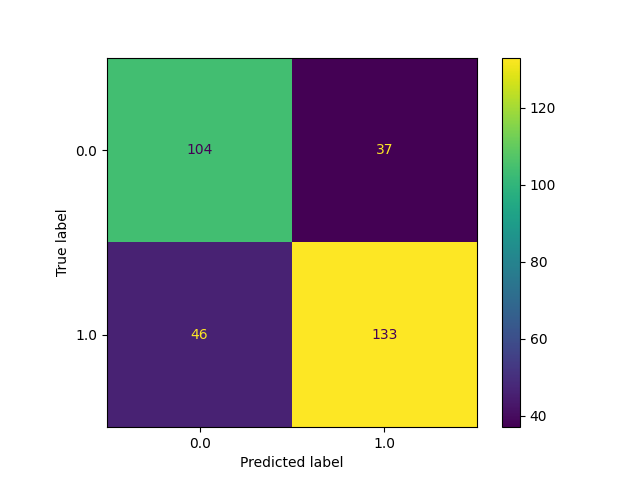
\includegraphics[width=0.95\textwidth]{conMatBinary.png}
	\caption{Binary}
	\label{fig:logo}
\end{figure}
\begin{figure}[h]
	\centering
	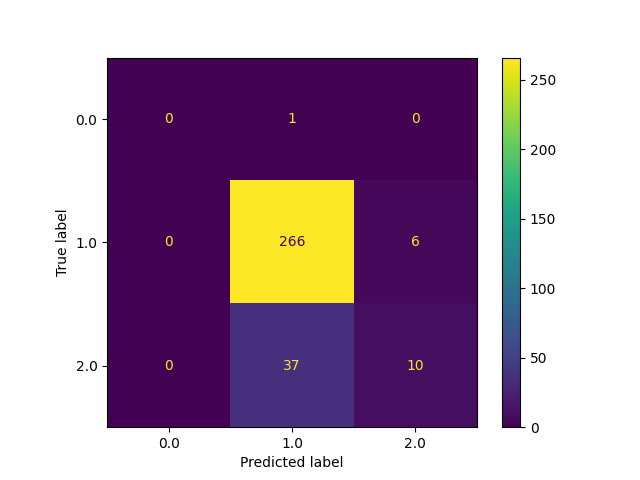
\includegraphics[width=0.95\textwidth]{conMatMulti.png}
	\caption{Multi-Class}
	\label{fig:logo}
\end{figure}	 
\begin{figure}[h]
	\centering
	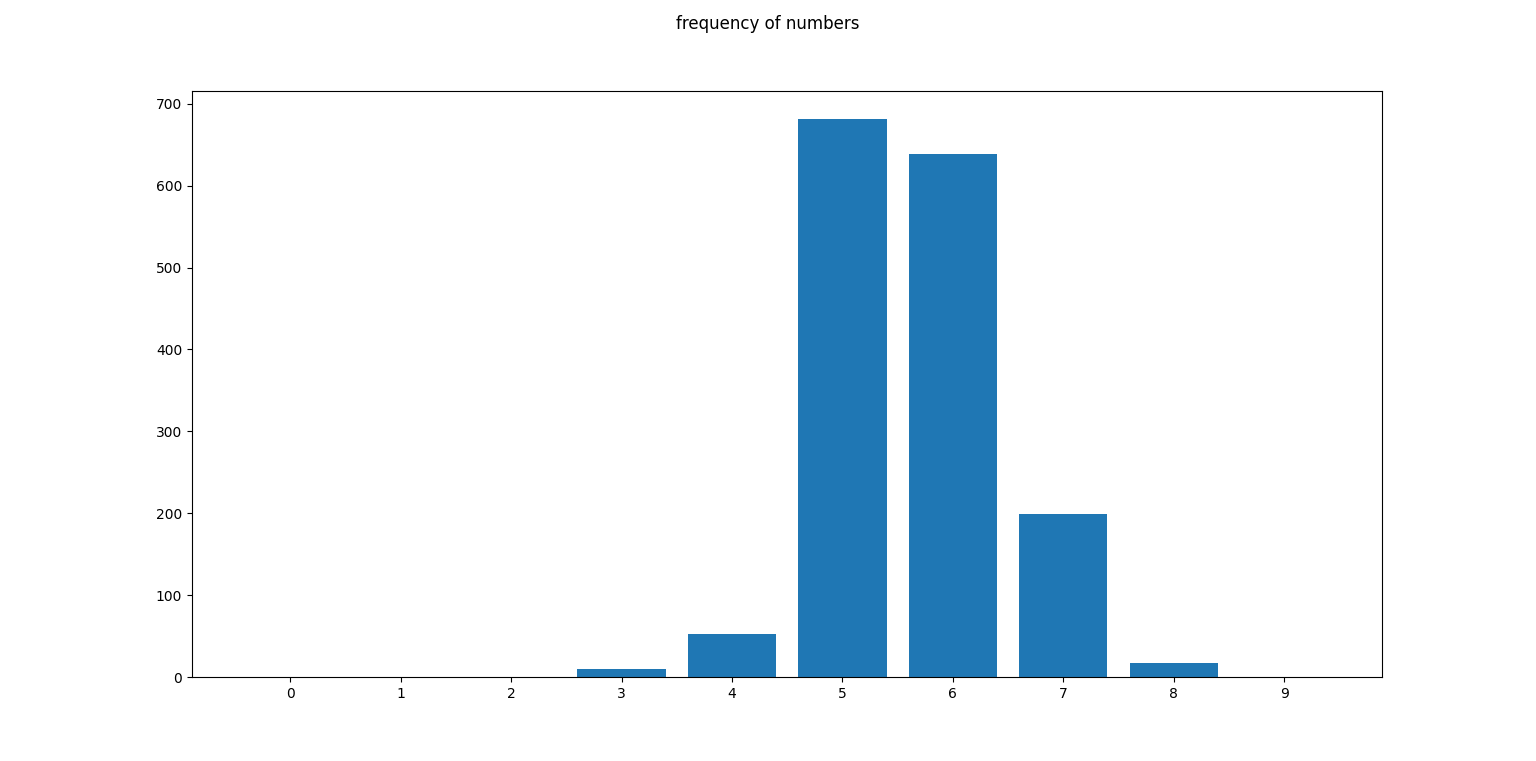
\includegraphics[width=0.95\textwidth]{freqNum.png}
	\caption{Numbers}
	\label{fig:logo}
\end{figure}

\end{document}